\subsection{Análisis de componentes principales}

Se aplico el algoritmo de PCA descrito en la sección \ref{sec:pca} con el kernel lineal, polinomial, gaussiano y sigmoide y los parámetros de la tabla \ref{table:pca_parameters}. En la figura \ref{fig:PCA_2d} se observan los resultados para el caso bidimensional.

\begin{figure}[H]
    \centering
    \begin{subfigure}{8.4cm}
        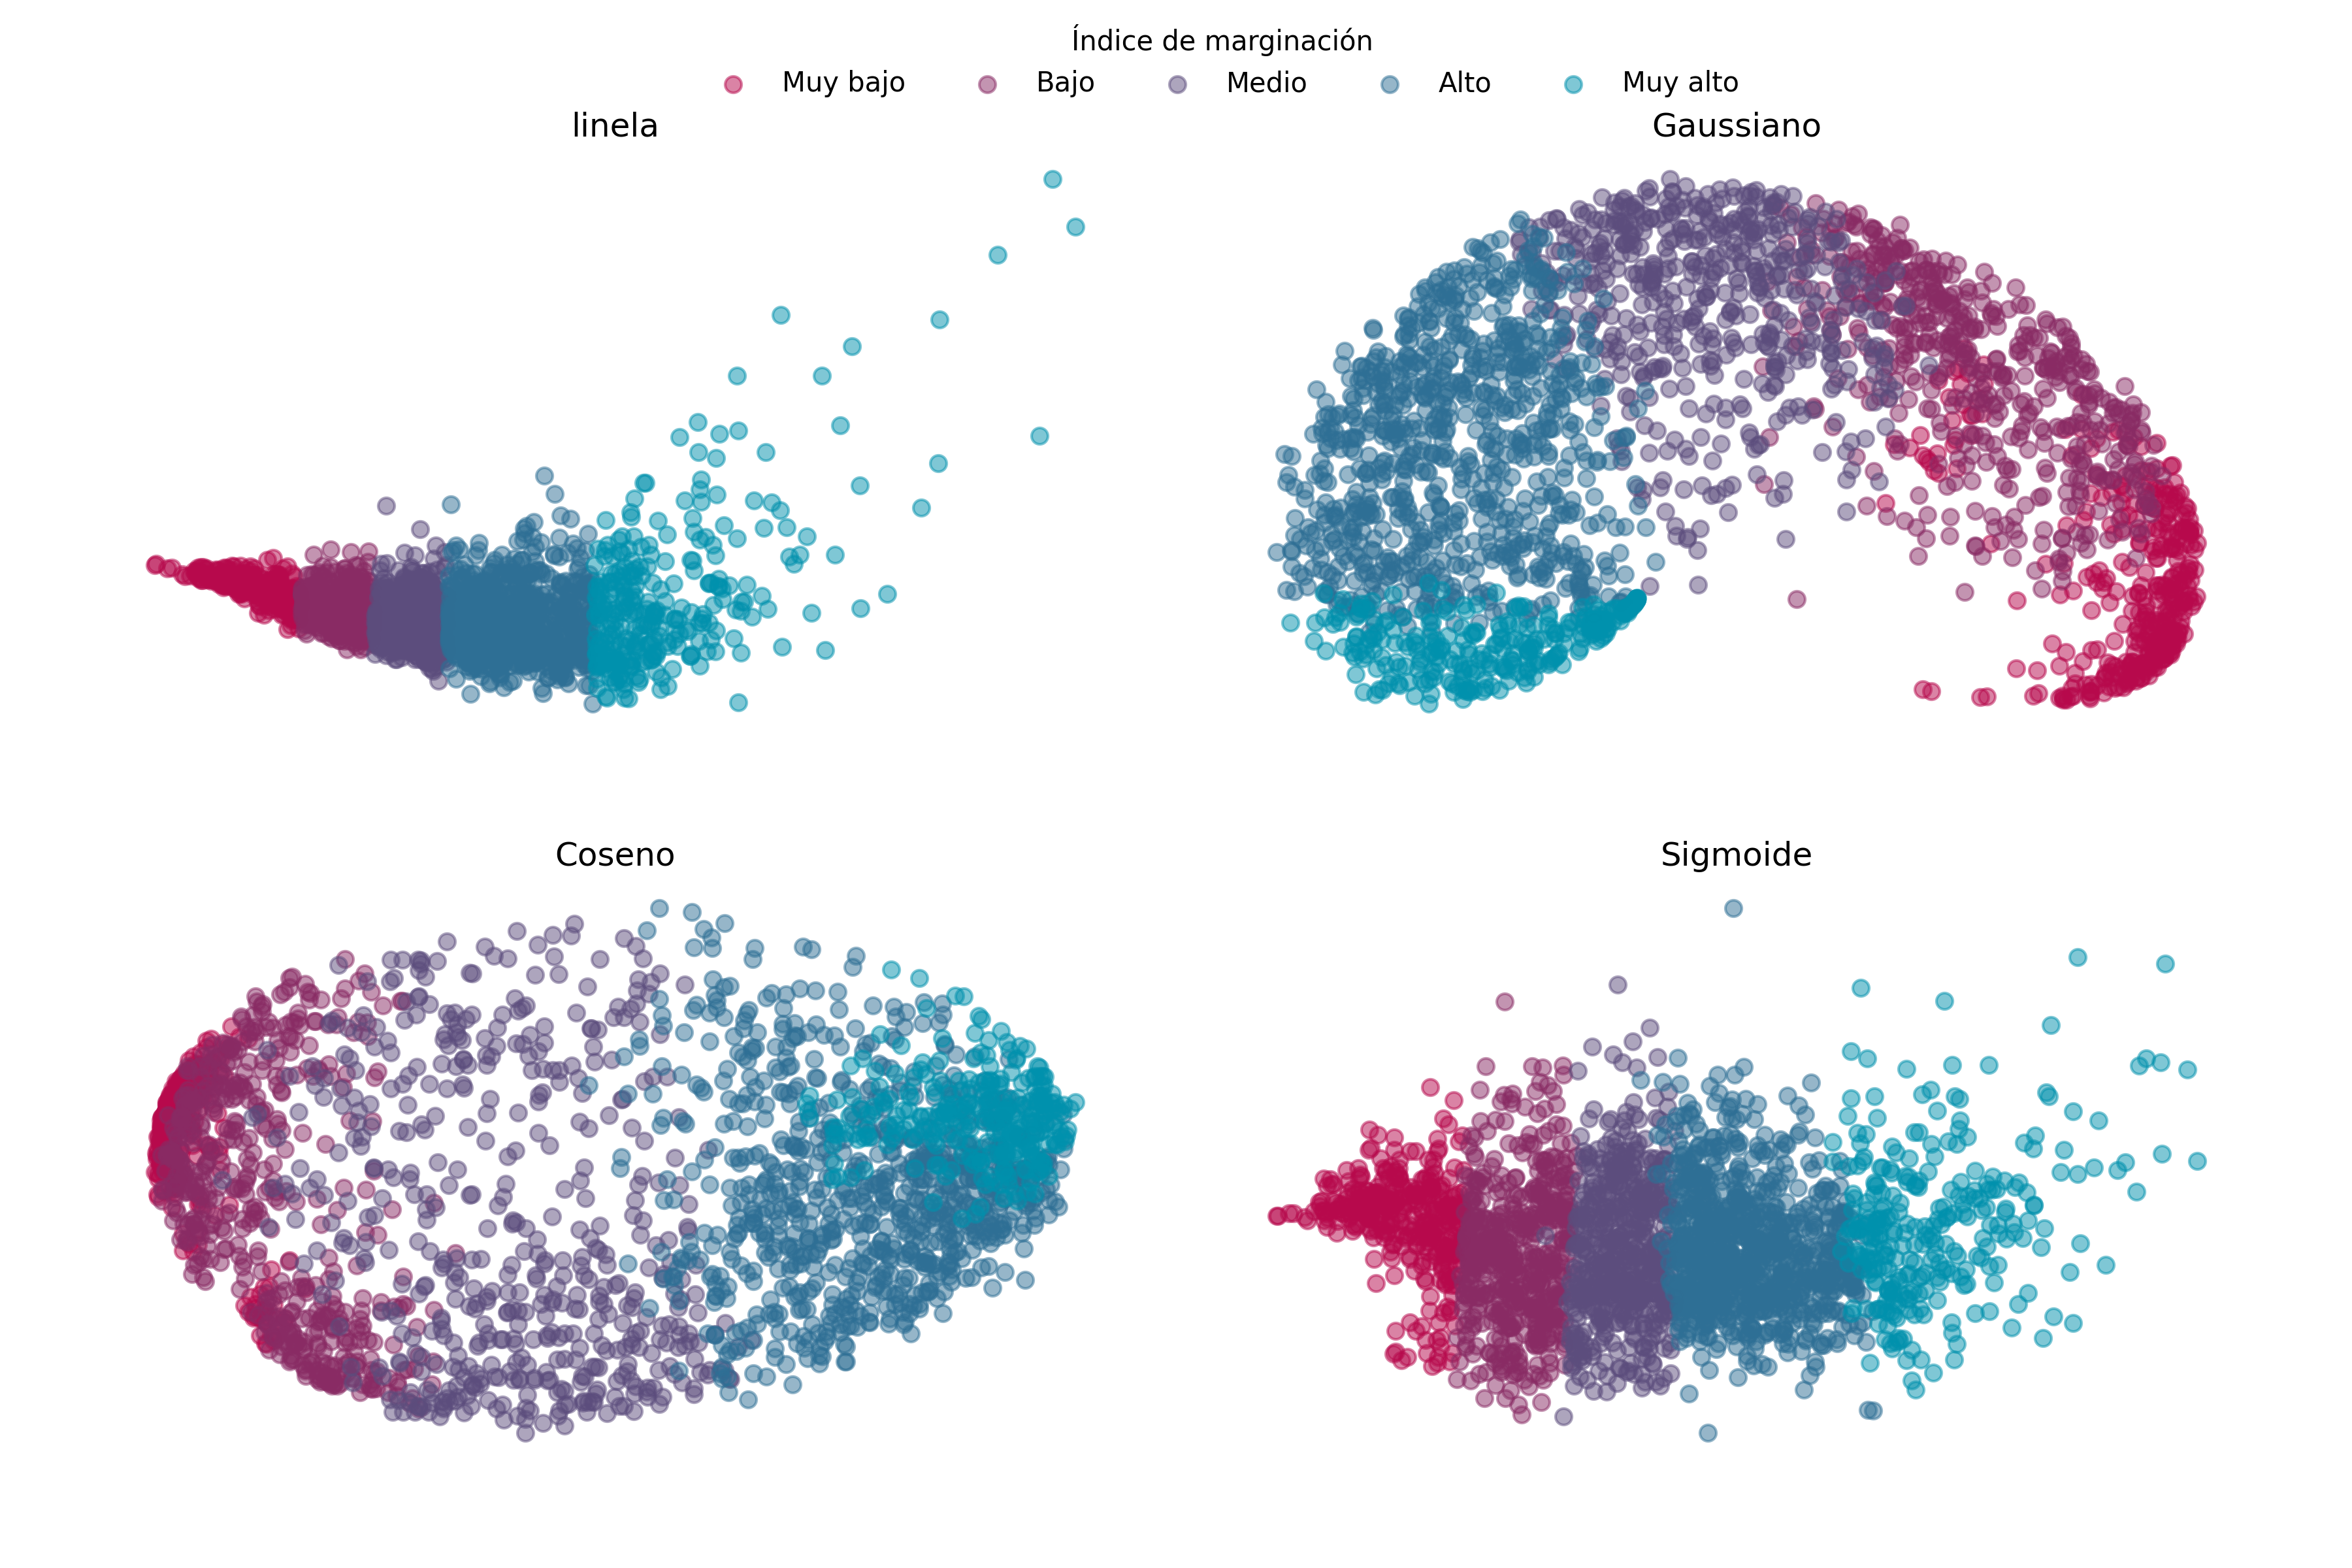
\includegraphics[width=1\linewidth]{Graphics/Data_2015/PCA_2D.png}
        \caption{Datos 2015}
    \end{subfigure}
    \begin{subfigure}{8.4cm}
        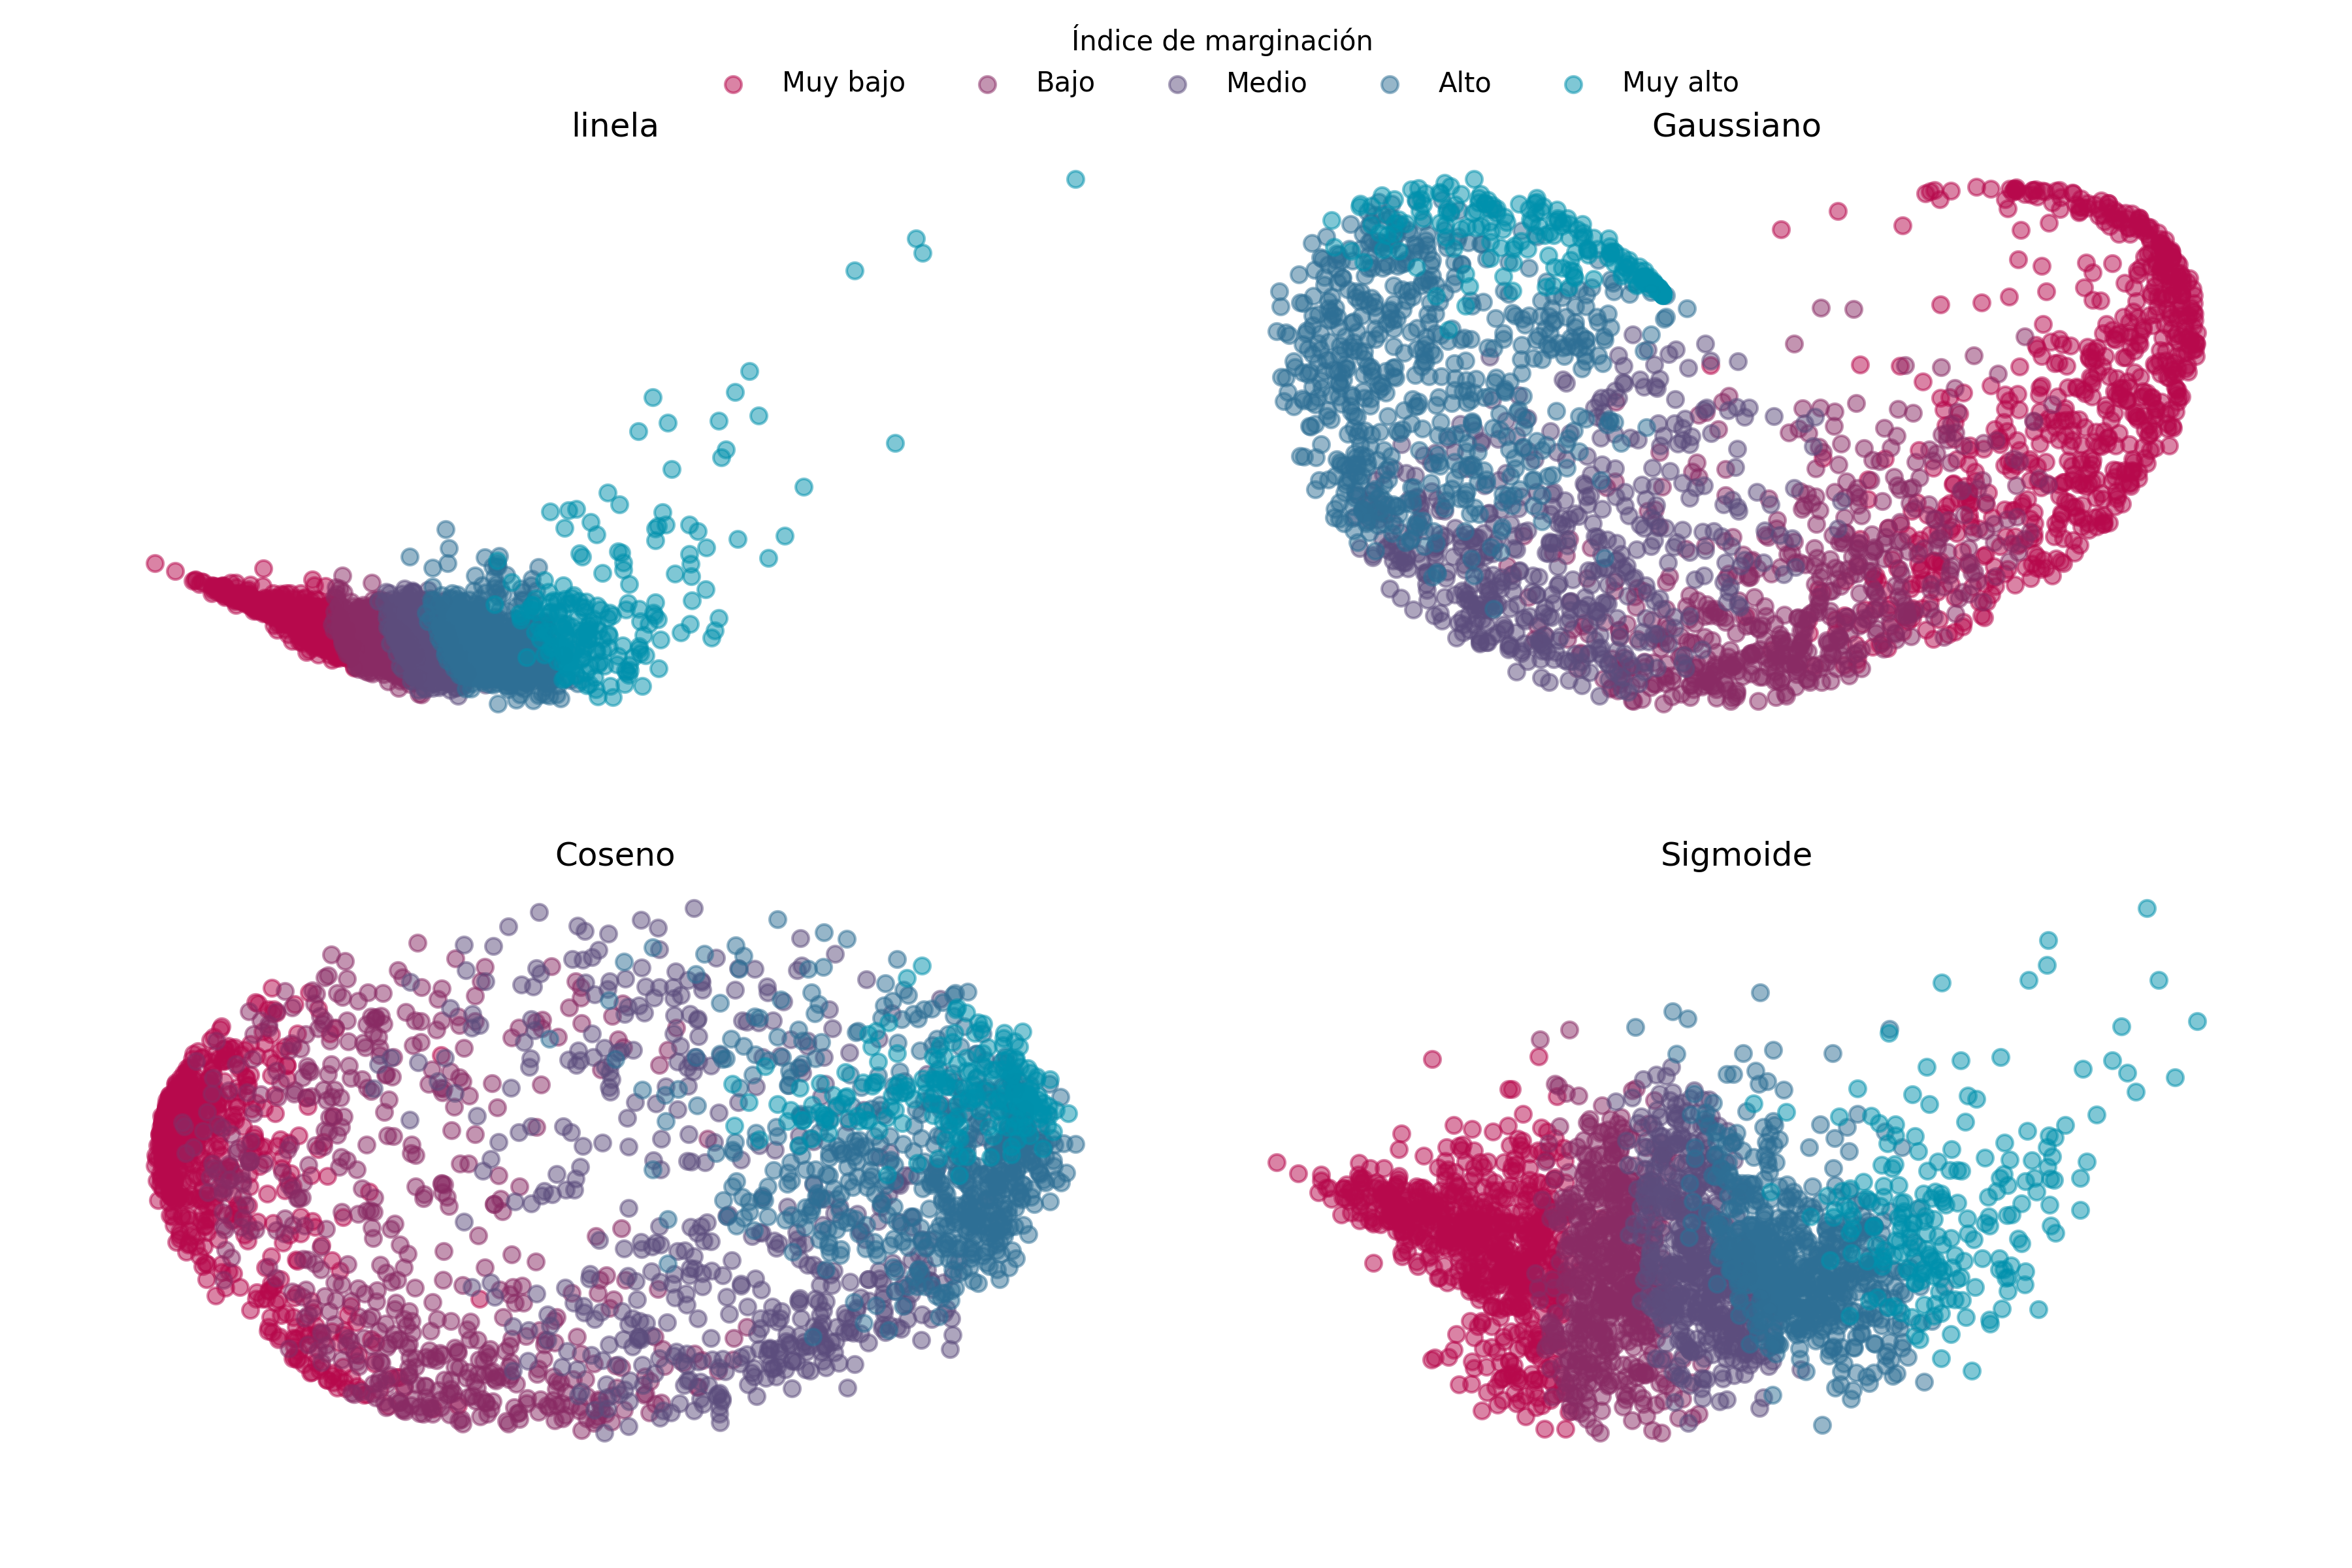
\includegraphics[width=1\linewidth]{Graphics/Data_2020/PCA_2D.png}
        \caption{Datos 2020}
    \end{subfigure}
    \caption{Resultados de aplicar PCA para el caso bidimensional para los datos de índice de marginación de los años 2015 y 2020.}
    \label{fig:PCA_2d}
\end{figure}

En la tabla \ref{table:pca_results} se pueden descargar las visualizaciones tridimensionales de los resultados del algoritmo PCA en el caso tridimensional.

\begin{table}[H]
    \centering
    \begin{tabular}{lrr} \hline
        \multirow{2}{*}{Kernel} & \multicolumn{2}{c}{Años}                                                                                                                                                                                                                                                    \\ \cline{2-3}
                                & 2015                                                                                                                                 & 2020                                                                                                                                 \\ \hline
        Lineal                  & \href{https://github.com/giovannilopez9808/Reconocimiento_de_patrones_proyecto/raw/main/Graphics/Data_2015/PCA_3D_linear.mp4}{Link}  & \href{https://github.com/giovannilopez9808/Reconocimiento_de_patrones_proyecto/raw/main/Graphics/Data_2020/PCA_3D_linear.mp4}{Link}  \\
        Coseno                  & \href{https://github.com/giovannilopez9808/Reconocimiento_de_patrones_proyecto/raw/main/Graphics/Data_2015/PCA_3D_cosine.mp4}{Link}  & \href{https://github.com/giovannilopez9808/Reconocimiento_de_patrones_proyecto/raw/main/Graphics/Data_2020/PCA_3D_cosine.mp4}{Link}  \\
        Gaussiano               & \href{https://github.com/giovannilopez9808/Reconocimiento_de_patrones_proyecto/raw/main/Graphics/Data_2015/PCA_3D_rbf.mp4}{Link}     & \href{https://github.com/giovannilopez9808/Reconocimiento_de_patrones_proyecto/raw/main/Graphics/Data_2020/PCA_3D_rbf.mp4}{Link}     \\
        Sigmode                 & \href{https://github.com/giovannilopez9808/Reconocimiento_de_patrones_proyecto/raw/main/Graphics/Data_2015/PCA_3D_sigmoid.mp4}{Link} & \href{https://github.com/giovannilopez9808/Reconocimiento_de_patrones_proyecto/raw/main/Graphics/Data_2020/PCA_3D_sigmoid.mp4}{Link} \\ \hline
    \end{tabular}
    \caption{Link de descarga para las visualizaciones tridimensionales de los resultados de PCA para el kernel lineal, coseno, gaussiano y sigmoide en los años 2015 y 2020.}
    \label{table:pca_results}
\end{table}